\documentclass[14pt]{extarticle}
\def\activityid{F03-K-v2}\usepackage[letterpaper,margin=.65in,top=.60in,bottom=.65in]{geometry}
\usepackage[T1]{fontenc}\usepackage[default]{sourcesanspro}
\usepackage{microtype,tikz,array,tabularx,fancyhdr,amsmath,amssymb}
\usepackage[hidelinks]{hyperref}\usetikzlibrary{calc,arrows.meta}
\setlength{\parindent}{0pt}\setlength{\parskip}{7pt}\setlength{\headheight}{0pt}\setlength{\footskip}{26pt}
\setlength{\emergencystretch}{2em}\pagestyle{fancy}\fancyhf{}\renewcommand{\headrulewidth}{0pt}\renewcommand{\footrulewidth}{.4pt}
\fancyfoot[L]{\scriptsize Bellingham Math Circle / Week 3 / \activityid}\fancyfoot[R]{\scriptsize \thepage}
\definecolor{ink}{gray}{.12}\definecolor{soft}{gray}{.95}\color{ink}
\newcommand{\PageTitle}[2]{{\fontsize{10}{12}\selectfont\bfseries WEEK 3\quad CODE MACHINES\hfill #1\par}\vspace{3pt}{\fontsize{26}{29}\selectfont\bfseries #2\par}\vspace{2pt}}
\newcommand{\NameLine}{{\small Name: \rule{2.65in}{.4pt}\hfill Date: \rule{1.35in}{.4pt}\par}\vspace{4pt}}
\newcommand{\Task}[2]{\par\vspace{3pt}{\large\bfseries #1}\par #2\par}
\newcommand{\Subhead}[1]{\par\vspace{3pt}{\large\bfseries #1}\par}
\newcommand{\RuleBox}[1]{\par\begingroup\setlength{\fboxsep}{8pt}\colorbox{soft}{\parbox{\dimexpr\linewidth-16pt\relax}{#1}}\endgroup\par}
\newcommand{\WriteBox}[2]{\par\textbf{#1}\par\vspace{2pt}\begin{tikzpicture}\draw[black!40,line width=.5pt] (0,0) rectangle (\dimexpr\linewidth-.5pt\relax,#2);\end{tikzpicture}\par}
\newcommand{\StudentFooter}{\vfill{\small Try it with objects. Explain by pointing, talking, or drawing.}\par}
\newcommand{\LampRing}[3]{\begin{tikzpicture}[x=1in,y=1in]
\foreach \i in {1,...,#1}{\coordinate (v\i) at ({90-360*(\i-1)/#1}:#2);}
\foreach \i in {1,...,#1}{\pgfmathtruncatemacro{\j}{mod(\i,#1)+1}\draw[thick] (v\i)--node[midway,fill=white,inner sep=2pt,font=\small]{\i\j}(v\j);}
\foreach \i in {1,...,#1}{\node[circle,draw,fill=white,minimum size=.52in,inner sep=0pt,font=\bfseries] at(v\i){\i};}
\foreach \i in {#3}{\node[circle,draw,fill=ink,text=white,minimum size=.52in,inner sep=0pt,font=\bfseries] at(v\i){\i};}
\end{tikzpicture}}
\newcommand{\Lights}[1]{\begin{tikzpicture}[x=.55in,y=.55in,baseline=-.10in]\foreach \v [count=\i] in {#1}{\ifnum\v=1\fill (\i,0) circle(.16in);\else\draw (\i,0) circle(.16in);\fi}\end{tikzpicture}}
\newcommand{\ClockRing}[2]{\begin{tikzpicture}[x=1in,y=1in]\draw[black!30] (0,0) circle(#2);\pgfmathtruncatemacro{\n}{#1-1}\foreach\i in {0,...,\n}{\node[circle,draw,fill=white,minimum size=.35in,inner sep=0pt] at({90-360*\i/#1}:#2){\i};}\draw[-{Stealth},thick] (-.35,.15) arc(155:25:.38);\node[font=\small] at(0,-.18){clockwise};\end{tikzpicture}}
\newcommand{\Key}[2]{\begin{center}\renewcommand{\arraystretch}{1.55}\begin{tabular}{c|*{#1}{c}}in&#2\end{tabular}\end{center}}

\begin{document}

\PageTitle{K--1 / 1}{The changing-symbol machine}\NameLine
\RuleBox{One turn changes each symbol by the same key. Point, draw, or use symbol cards. Try making messages before using the key.}
\begin{center}{\LARGE
\begin{tabular}{c@{\quad$\longrightarrow$\quad}c}
$\bigcirc$&$\triangle$\\[10pt]$\triangle$&$\square$\\[10pt]$\square$&$\bigcirc$
\end{tabular}}\end{center}
\Task{1. Send it through.}{What comes out of this message? Read one symbol at a time.}
\begin{center}{\Huge\(\bigcirc\quad\triangle\quad\bigcirc\)}\end{center}
\WriteBox{My new message (draw or place cards):}{.7in}
\Task{2. Run it backward.}{Your friend receives \(\square\). What went in? Can you point backward along an arrow to check? Try each symbol.}
\WriteBox{Make a message for someone else to decode.}{.8in}
\StudentFooter
\newpage
\PageTitle{K--1 / 2}{When does it come home?}
\Task{3. Keep going!}{Put a counter on the circle. Follow one arrow each turn. How many turns before it first comes back? Try starting at a different symbol.}
\begin{center}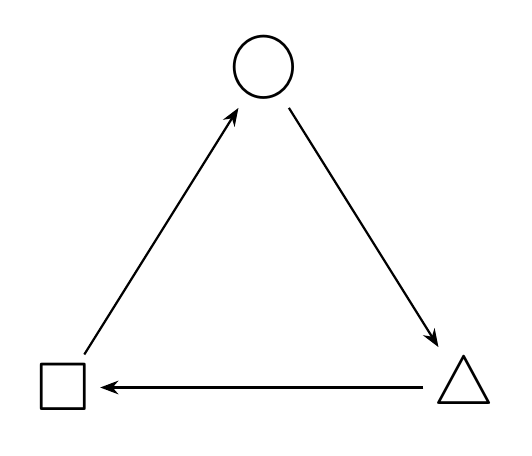
\begin{tikzpicture}[x=1in,y=1in,every node/.style={font=\Huge}]
\node(A)at(0,1){$\bigcirc$};\node(B)at(1,-.6){$\triangle$};\node(C)at(-1,-.6){$\square$};
\draw[-{Stealth},thick](A)--(B);\draw[-{Stealth},thick](B)--(C);\draw[-{Stealth},thick](C)--(A);
\end{tikzpicture}\end{center}
\Task{4. Change the key.}{Now circle becomes triangle, triangle becomes circle, and square stays square. Will all symbols come home together after two turns? Show it with three counters.}
\WriteBox{Adult: record the child's experiment or explanation.}{1in}
\textbf{Try a broken key:} If circle and triangle both become square, can a receiver know which one you sent?
\StudentFooter

\end{document}
